\jxhj{%教学后记
	}
\skrq{%授课日期
	2017年11月14日 4-5节}
\ktmq{%课题名称
	 型腔加工}
\jxmb{%教学目标,每行前面要加 \item
	\item 掌握型腔加工的下刀方式;
    \item 掌握矩形槽去残料的方式;
    \item 会用G91斜线下刀及Z向分层;
    \item 会编写矩形槽的程序。}
\jxzd{%教学重点,每行前面要加 \item
	\item 用G91斜线下刀及Z向分层;
	\item 编写矩形槽的程序。 }
\jxnd{%教学难点,每行前面要加 \item
	\item 编写矩形槽的程序。 }
\jjff{%教学方法
	通过讲述、举例、演示法来说明;}

\makeshouye %制作教案首页

%%%%教学内容
\subsection{组织教学}
\begin{enumerate}[\hspace{2em}1、]
	\item 集中学生注意力;
	\item 清查学生人数;
	\item 维持课堂纪律;
\end{enumerate}

\subsection{复习导入及主要内容}
\begin{enumerate}[1、]
\item 刀具的选择;
\item 下刀方式;
\item 斜线下刀;
\item 去残料方式;
\item 圆形槽铣削加工实例。
\end{enumerate}

\subsection{教学内容及过程}
\subsubsection{方形槽铣削}
利用数控铣床加在\diameter 110*35的毛坯上加工80*60深5mm的方槽。毛坯材料为45号钢,上表面未加工。按图样要求完成零件的节点、基点、辅助点计算。设定工件坐标系,制定正确的工艺方案(包括定位,夹紧方案和工艺路线),选择合理的刀具和切削工艺参数,编写数控加工程序。

\begin{figure}[h]
	\centering
	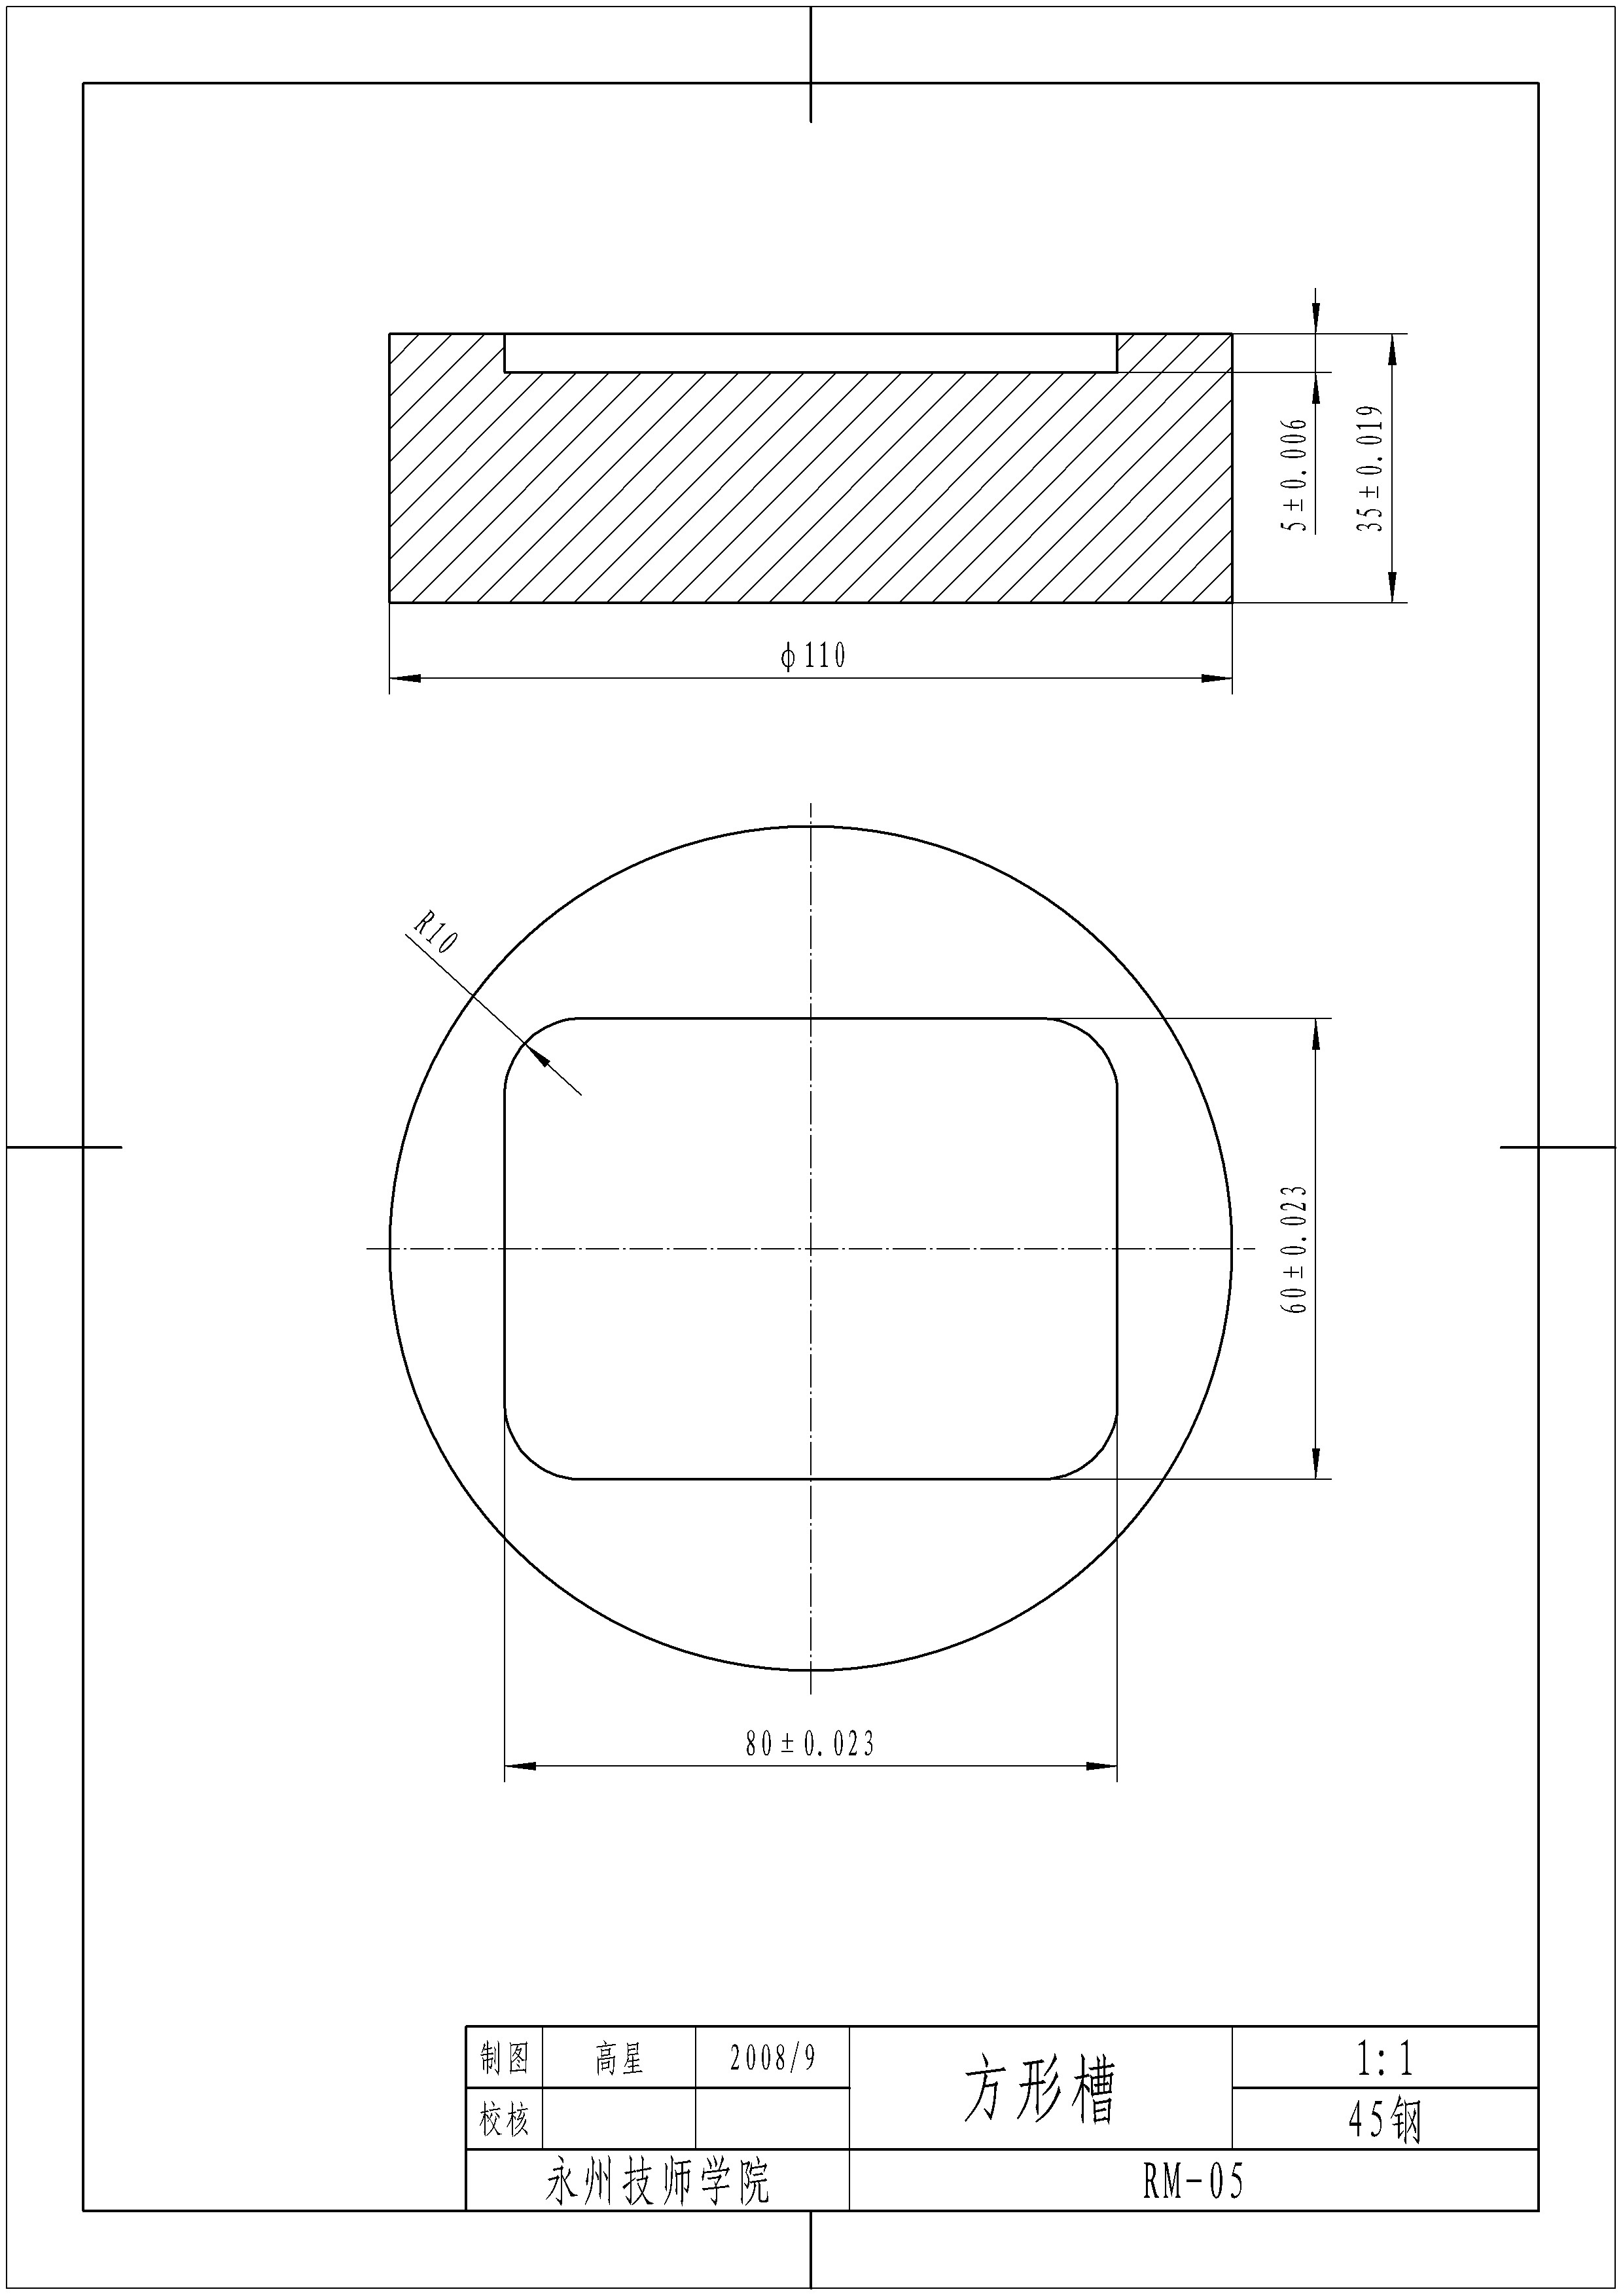
\includegraphics[width=0.8\linewidth,trim=130 180 80  120,clip]{data/image/18-1.jpg}
	\caption{方形槽铣削}
	\label{fig:18-1}
\end{figure}

1、工艺分析:

零件简单,尺寸精度均达到IT8-IT7级

采用机用平口钳装夹,两侧面先工艺平面用于装夹

工件坐标系原点设在铣好的上表面中心

工序:平面

挖槽:

2、刀具选择:

平面用\diameter 80可转位铣刀,

挖槽:粗加工用\diameter 14三刃立铣刀

精加工用\diameter 12四刃立铣刀

3、刀削参数的铣铣择:

{\noindent
    
    \begin{figure}[!hbtp]
        \centering
        \footnotesize
        %\hspace{-3.4ex}
        \renewcommand\arraystretch{1.9}
        \begin{tabu}to 0.6\textwidth{|c|c|c|c|c|c|c|c|}
            \hline 
            序号 & 加工 & 刀具类型 & 刀具 & 主轴 & 进给& 长度 & 半径 \\ 
            & 内容 &  & 材料 & 转速 & 速度 & 补偿 & 补偿 \\
            \hline 
            1 & 粗加工上表面 & \diameter 可转位铣刀 & 硬质合金 & 500 & 250 &  &  \\ 
            \hline 
            2&精加工上表面& \diameter 可转位铣刀  & 硬质合金 &800  &160  &  &  \\ 
            \hline 
            3&粗加工槽  & \diameter 14立铣刀 &高速钢  &500  &80  &  &7.2  \\ 
            \hline 
            4&精加工槽  & \diameter 12立铣刀 &高速钢  &800  &80  &  &5.985  \\ 
            \hline 
        \end{tabu} 
\end{figure}}

4、走刀路径

粗加工刀补:7.2  

5、参考程序

\begin{lstlisting}
O1;
G54G17G90G40;
M3S400;
G1Z100.0F2000;
X-30.0Y20.0;
Z5.0;
G1Z0F150.0;
M98P2;
G1Z100.0F2000;
M5;
M30;
\end{lstlisting}

\begin{lstlisting}
O2;
G91G1X60.0Z-5.0F40;
X-60.0F150;
M98P200;
G90G1X25.0Y0
D1M98P2000
G1X-30.0Y20.0
M99
\end{lstlisting}
\begin{lstlisting}
O200;
G91G1Y-12.0
X60.0
Y-12.0
X-60.0
Y-12.0
X60.0;
Y-4.0
X-60.0
M99
\end{lstlisting}
\begin{lstlisting}
O2000;
G1G41X30.0Y10.0
G3X40.0Y0R10.0
G1Y20.0
G3X30.0Y30.0R10.0
G1Y-20.0
G3X-30.0Y-30.0R10.0
G1X30.0
G3X40.0Y-20.0
G1Y0
G3X30.0Y10.0R10.0
G1G40X25.0Y0
M99
\end{lstlisting}
课堂练习:
如果加工深度为12mm,怎样写程序:
\begin{figure}[h]
    \centering
    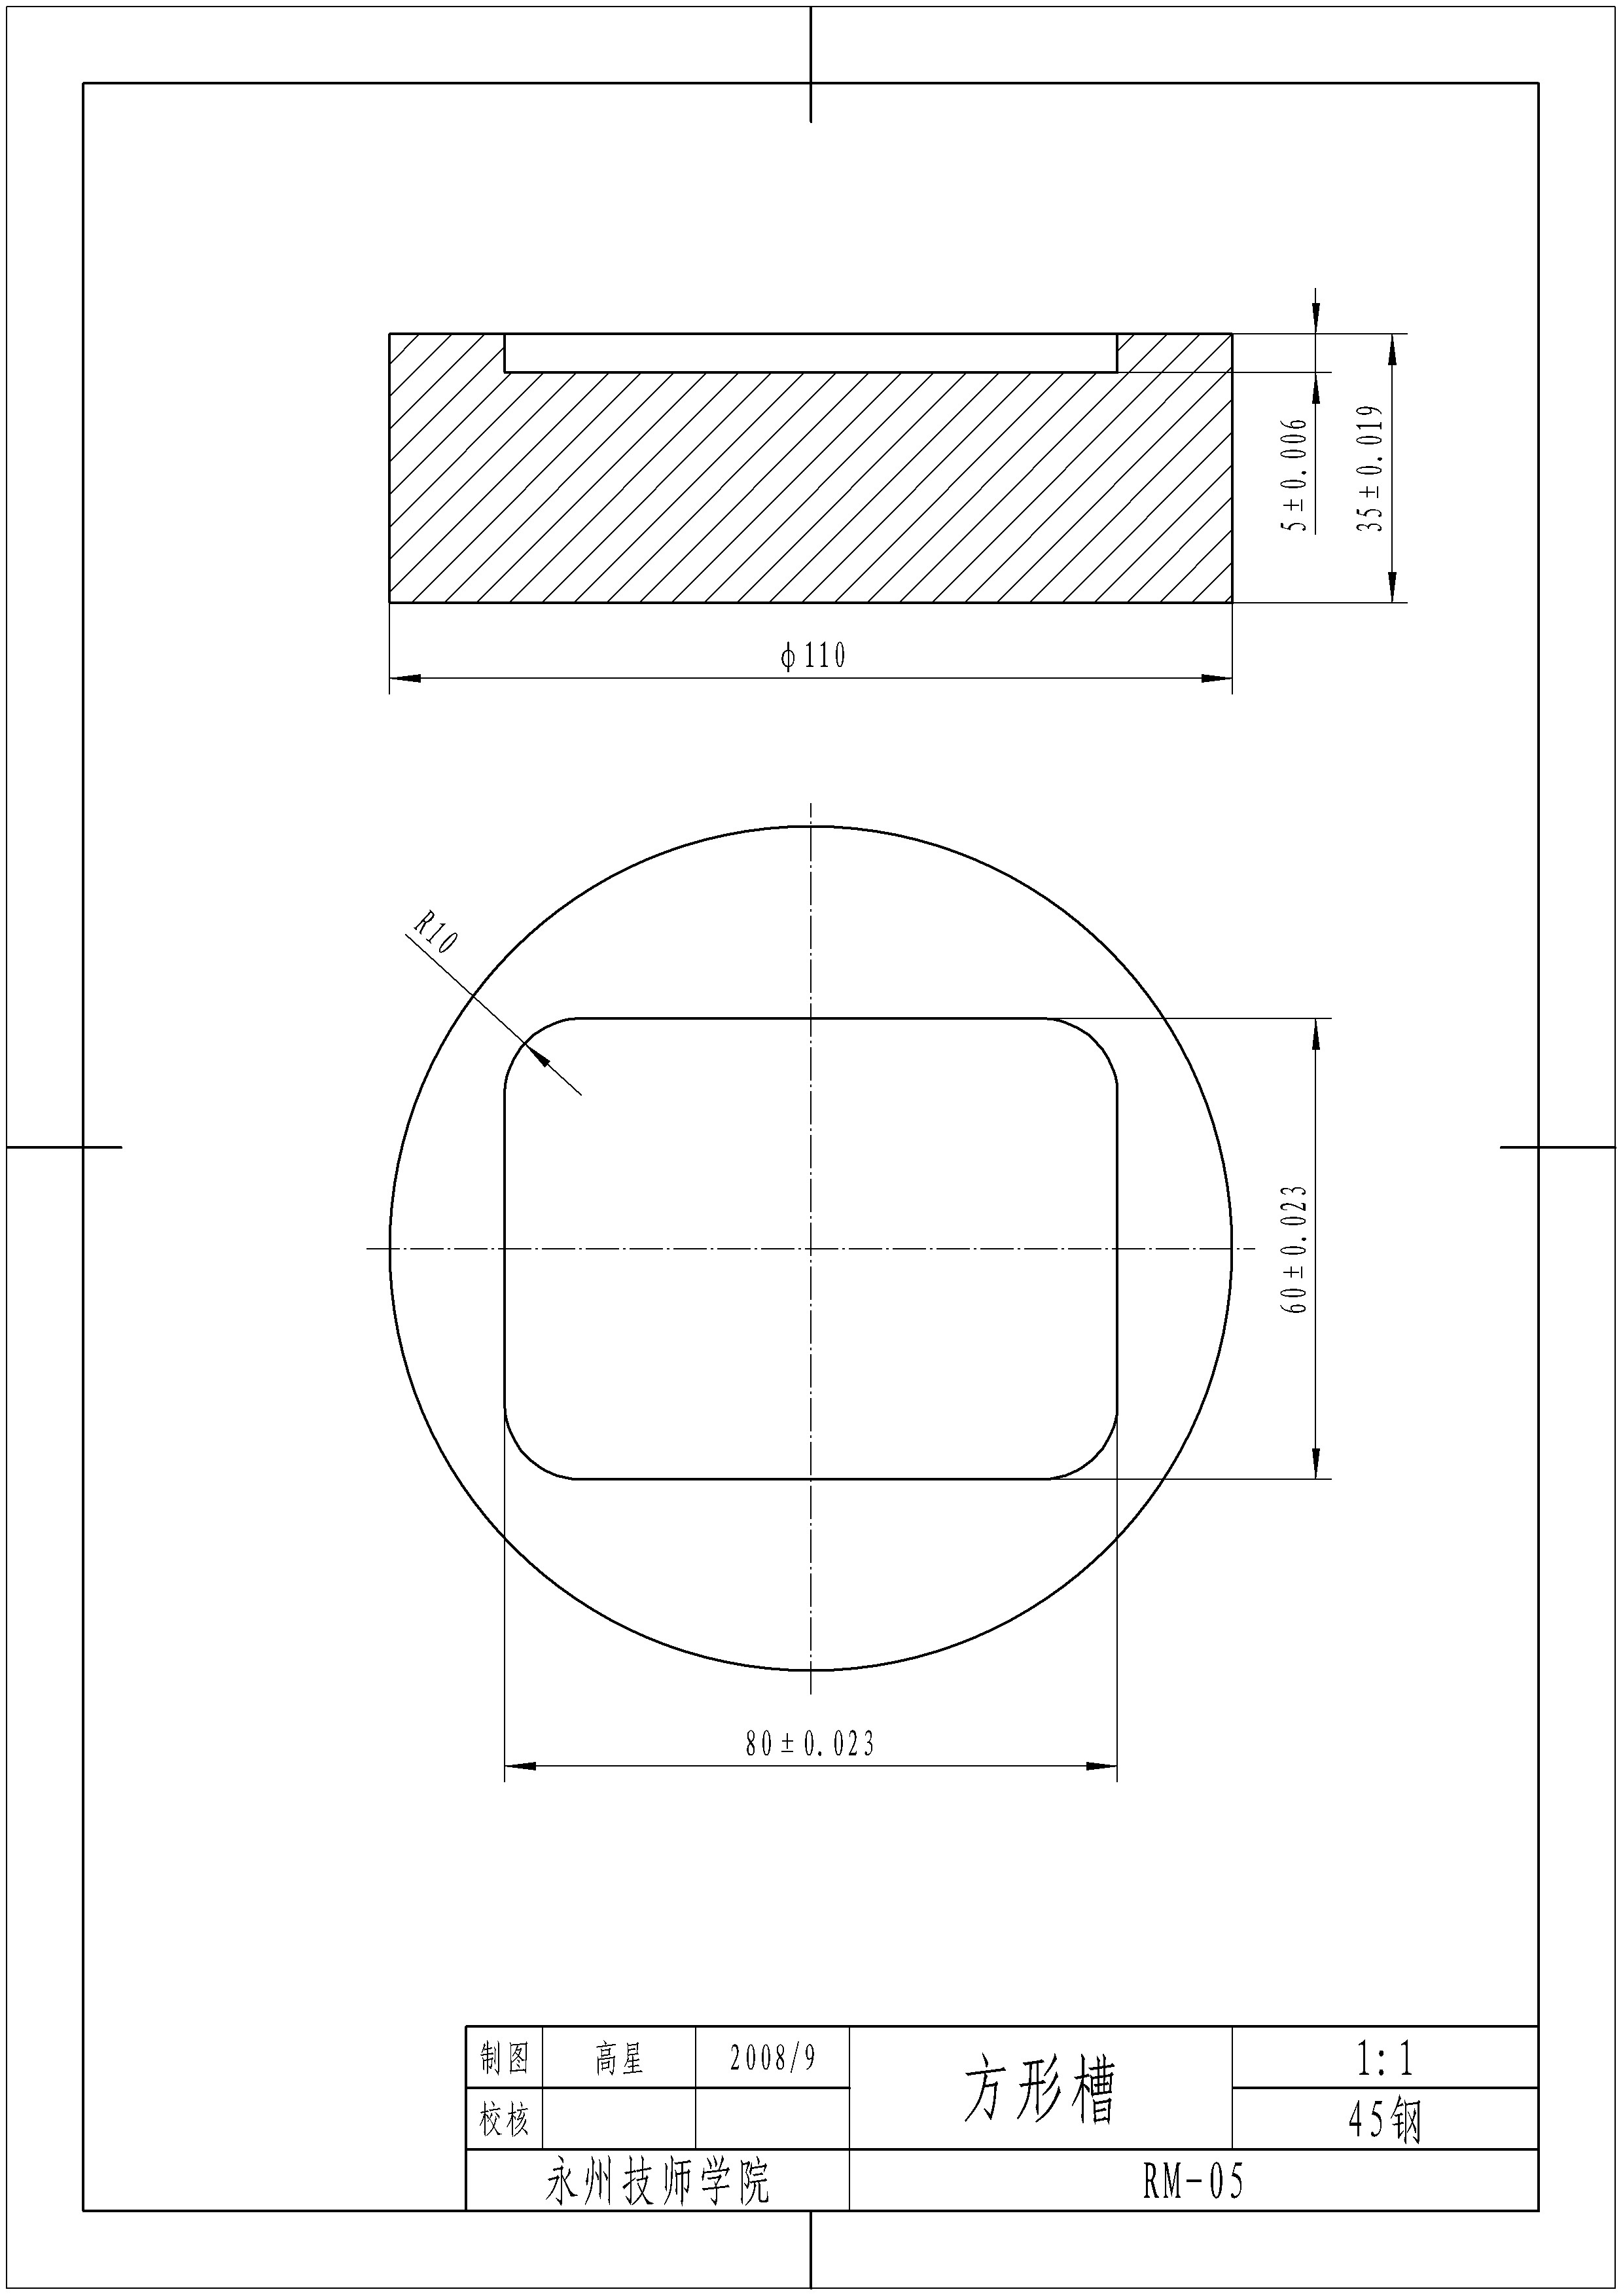
\includegraphics[width=0.8\linewidth,trim=130 180 80  120,clip]{data/image/18-1.jpg}
    \caption{方形槽铣削,深度改为12mm}
    \label{fig:18-2}
\end{figure}


\subsection{课堂小结}
\begin{enumerate}[1、]
\item 刀具的选择;
\item 下刀方式;
\item 斜线下刀;
\item 去残料方式;
\item 方槽铣削加工实例。
\end{enumerate}

\vfill
\subsection{布置作业}
\begin{enumerate}[1、]
	\item 编写上面的程序。
\end{enumerate}
\vfill